% Created 2022-01-23 Sun 15:22
% Intended LaTeX compiler: pdflatex
\documentclass[10pt, compress]{beamer}
\usepackage[utf8]{inputenc}
\usepackage[T1]{fontenc}
\usepackage{graphicx}
\usepackage{longtable}
\usepackage{wrapfig}
\usepackage{rotating}
\usepackage[normalem]{ulem}
\usepackage{amsmath}
\usepackage{amssymb}
\usepackage{capt-of}
\usepackage{hyperref}
\institute[Mannodi Group]{Purdue Materials Science and Engineering
\inst{1} Mannodi Group
\mode<beamer>{\usetheme{Warsaw}}
\useoutertheme{miniframes}
\usetheme{default}
\author{Panayotis Manganaris\inst{1}}
\date{\today}
\title{A High-Throughput Computational Dataset of Halide Perovskite Alloys}
\hypersetup{
 pdfauthor={Panayotis Manganaris\inst{1}},
 pdftitle={A High-Throughput Computational Dataset of Halide Perovskite Alloys},
 pdfkeywords={},
 pdfsubject={},
 pdfcreator={Emacs 27.2 (Org mode 9.5)}, 
 pdflang={English}}
\begin{document}

\maketitle
\begin{frame}{Outline}
\tableofcontents
\end{frame}

\expandafter\def\expandafter\insertshorttitle\expandafter{%
  \insertshorttitle\hfill
  \insertframenumber\,/\,\inserttotalframenumber}
\section{Methodology}
\label{sec:orga06c6e6}
\begin{frame}[fragile,allowframebreaks]{DFT Details}
 \begin{block}{figure 1-a ::}
a) Perovskite structure summary
b) pie-chart showing every species representation in DFT dataset
c) flowchart of workflow
\end{block}
\begin{block}{figure 2}
a, b, c, d -- figures showing relations between primary outputs
\begin{block}{computational vs empirical bad gaps}
\end{block}
\begin{block}{plot}
\begin{verbatim}
---------------------------------------------------------------------------
NameError                                 Traceback (most recent call last)
/tmp/ipykernel_22940/1552246790.py in <module>
      1 fig, ax = plt.subplots(figsize=[10,10])
----> 2 ax.scatter(comparision_df.EMP_bg_eV, comparision_df.PBE_bg_eV)
      3 ax.set_title("test")
      4 ax.set_xlabel("EMP")
      5 ax.set_ylabel("PBE")

NameError: name 'comparision_df' is not defined
\end{verbatim}

\begin{center}
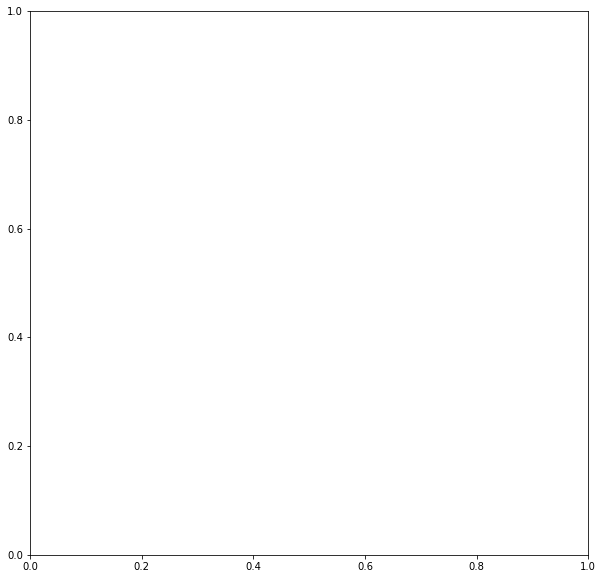
\includegraphics[width=.9\linewidth]{./.ob-jupyter/2d80835aef2211297f37b26050fad6e2821feb9b.png}
\end{center}
\end{block}
\end{block}
\end{frame}

\subsection{Accessing and Analyzing DFT Data}
\label{sec:orgeda3a30}
\begin{frame}[label={sec:orgd94e261}]{Collect experimental points}
\begin{description}
\item[{figure 3}] rigorous experimental comparison
see prof K's expt\textsubscript{data.xlsx} -- extract 14D chem-comp and band gap and lattice constant.
there's quite a few Perovskite compositions with reported BG and other solar cell performance parameters

\begin{itemize}
\item build the perovskites database and make scripts to build it.
\end{itemize}
\end{description}
\end{frame}
\begin{frame}[label={sec:orgb29d565}]{}
\begin{description}
\item[{figure 4}] pearson maps
\end{description}
\end{frame}
\begin{frame}[label={sec:org66d96df}]{}
\end{frame}

\subsection{Data Visualization Methods}
\label{sec:org2066d0f}
\begin{frame}[label={sec:orgfc43b57}]{PCA examinations}
\begin{itemize}
\item 
\end{itemize}
\end{frame}
\begin{frame}[label={sec:orge4cdeb7}]{MDS, TSNE, ISOMAP, UMAP}
\begin{itemize}
\item 
\end{itemize}
\newpage
\end{frame}
\section{Results and discussion}
\label{sec:org4b81515}
\subsection{Visualization of DFT Data}
\label{sec:orgf0653fc}
\ldots{}\\
\newpage
\section{Perspective and Future Work}
\label{sec:orgc24c232}
\ldots{}\\

\section{figure ideas}
\label{sec:org147b24d}
\begin{enumerate}
\item compare exp with comp band gaps graphically
\item show distributions of measured outputs vs time and vs composition ratios?
\item show frequency of investigation over time (as in paper)
\item show change in band gap with multidimensional ratio shift
\end{enumerate}
\end{document}